%------------------------------------------------------------------------------%
\documentclass[fleqn,aspectratio=169,12pt]{beamer}

\usepackage{gaal}

\title{Definição Geométrica e Algébrica das Cônicas}

%------------------------------------------------------------------------------%
\begin{document}

\addtitle

%------------------------------------------------------------------------------%
\section{Interseções Entre um Plano e um Cone}

%------------------------------------------------------------------------------%
\begin{frame}{Cônicas}
  As cônicas são a interseção de um plano e um cone duplo
\end{frame}

%------------------------------------------------------------------------------%
\begin{frame}[t]{Cônicas}
\begin{columns}[t]
\column{0.5\linewidth}
  Seções cônicas
\column{0.5\linewidth}
  ~\\[-\baselineskip]
  \includegraphics{inter_cone}
\end{columns}
\end{frame}

%------------------------------------------------------------------------------%
\begin{frame}[t]{Cônicas}
\begin{columns}[t]
\column{0.5\linewidth}
  Seções cônicas
  \begin{itemize}
    \item Elipse
  \end{itemize}
\column{0.5\linewidth}
  ~\\[-\baselineskip]
  \includegraphics{inter_elipse}
\end{columns}
\end{frame}

%------------------------------------------------------------------------------%
\begin{frame}[t]{Cônicas}
\begin{columns}[t]
\column{0.5\linewidth}
  Seções cônicas
  \begin{itemize}
    \item Elipse \quad (círculo)
  \end{itemize}
\column{0.5\linewidth}
  ~\\[-\baselineskip]
  \includegraphics{inter_circulo}
\end{columns}
\end{frame}

%------------------------------------------------------------------------------%
\begin{frame}[t]{Cônicas}
\begin{columns}[t]
\column{0.5\linewidth}
  Seções cônicas
  \begin{itemize}
    \item Elipse \quad (círculo)
    \item Parábola
  \end{itemize}
\column{0.5\linewidth}
  ~\\[-\baselineskip]
  \includegraphics{inter_parabola}
\end{columns}
\end{frame}

%------------------------------------------------------------------------------%
\begin{frame}[t]{Cônicas}
\begin{columns}[t]
\column{0.5\linewidth}
  Seções cônicas
  \begin{itemize}
    \item Elipse \quad (círculo)
    \item Parábola
    \item Hipérbole
  \end{itemize}
\column{0.5\linewidth}
  ~\\[-\baselineskip]
  \includegraphics{inter_hiperbole}
\end{columns}
\end{frame}

%------------------------------------------------------------------------------%
\begin{frame}[t]{Cônicas}
\begin{columns}[t]
\column{0.5\linewidth}
  Seções cônicas
  \begin{itemize}
    \item Elipse \quad (círculo)
    \item Parábola
    \item Hipérbole
  \end{itemize}

  \bigskip
  Seções cônicas degeneradas
\column{0.5\linewidth}
  ~\\[-\baselineskip]
  \includegraphics{inter_cone}
\end{columns}
\end{frame}
%------------------------------------------------------------------------------%
\begin{frame}[t]{Cônicas}
\begin{columns}[t]
\column{0.5\linewidth}
  Seções cônicas
  \begin{itemize}
    \item Elipse \quad (círculo)
    \item Parábola
    \item Hipérbole
  \end{itemize}

  \bigskip
  Seções cônicas degeneradas
  \begin{itemize}
    \item Retas concorrentes
  \end{itemize}
\column{0.5\linewidth}
  ~\\[-\baselineskip]
  \includegraphics{inter_retas_concorrentes}
\end{columns}
\end{frame}

%------------------------------------------------------------------------------%
\begin{frame}[t]{Cônicas}
\begin{columns}[t]
\column{0.5\linewidth}
  Seções cônicas
  \begin{itemize}
    \item Elipse \quad (círculo)
    \item Parábola
    \item Hipérbole
  \end{itemize}

  \bigskip
  Seções cônicas degeneradas
  \begin{itemize}
    \item Retas concorrentes
    \item Reta
  \end{itemize}
\column{0.5\linewidth}
  ~\\[-\baselineskip]
  \includegraphics{inter_reta}
\end{columns}
\end{frame}

%------------------------------------------------------------------------------%
\begin{frame}[t]{Cônicas}
\begin{columns}[t]
\column{0.5\linewidth}
  Seções cônicas
  \begin{itemize}
    \item Elipse \quad (círculo)
    \item Parábola
    \item Hipérbole
  \end{itemize}

  \bigskip
  Seções cônicas degeneradas
  \begin{itemize}
    \item Retas concorrentes
    \item Reta
    \item Ponto
  \end{itemize}
\column{0.5\linewidth}
  ~\\[-\baselineskip]
  \includegraphics{inter_ponto}
\end{columns}
\end{frame}

%------------------------------------------------------------------------------%
\section{Definição Geométrica das Cônicas}

%------------------------------------------------------------------------------%
\begin{frame}{Cônicas}
  As cônicas são a interseção de um plano e um cone duplo
\end{frame}

%------------------------------------------------------------------------------%
\begin{frame}{Circunferência}
\begin{columns}
\column{0.4\textwidth}
  Uma \emph{circunferência}

  \pause
  é o conjunto dos pontos \(P\) do plano cuja distância
  a um ponto fixo \(C\) é constante \(r>0\)
\column{0.6\textwidth}
  \pause
  \begin{center}
  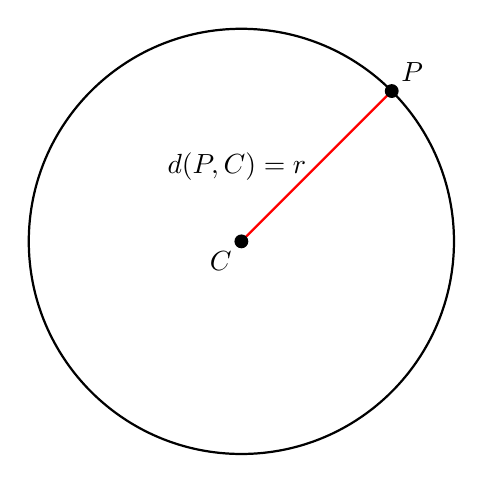
\begin{tikzpicture}[>=stealth]
    \draw[thick] (0,0) circle (2.7);

    \draw[red,thick] (0,0) -- node[black, left] {$d(P, C) = r$} (1.9092,1.9092);

    \fill (0,0)           circle (2.5pt) node[below  left] {$C$};
    \fill (1.9092,1.9092) circle (2.5pt) node[above right] {$P$};
  \end{tikzpicture}
  \end{center}
\end{columns}
\end{frame}

%------------------------------------------------------------------------------%
\begin{frame}{Elipse}
\begin{columns}
\column{0.4\textwidth}
  Uma \emph{elipse}

  \pause
  é o conjunto dos pontos \(P\) para os quais a soma das distâncias
  a dois pontos fixos \(F_1\) e \(F_2\) é constante

  \pause
  \bigskip
  Os pontos \(F_1\) e \(F_2\) são os focos
\column{0.6\textwidth}
  \pause
  \begin{center}
  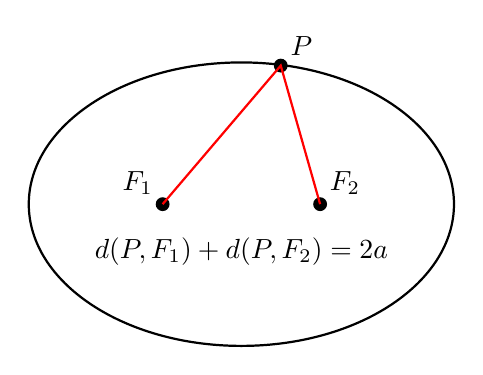
\begin{tikzpicture}[>=stealth]
    \draw[thick] (0,0) ellipse (2.7 and 1.8);

    \fill (-1,0)     circle (2.5pt) node[above left]  {$F_1$};
    \fill ( 1,0)     circle (2.5pt) node[above right] {$F_2$};
    \fill (0.5,1.76) circle (2.5pt) node[above right] {$P$};

    \draw[red,thick] (-1,0)--(0.5,1.76)--(1,0);

    \node at (0,-0.6) {$d(P,F_1)+d(P,F_2)=2a$};
  \end{tikzpicture}
  \end{center}
\end{columns}
\end{frame}

%------------------------------------------------------------------------------%
\begin{frame}{Parábola}
\begin{columns}
\column{0.4\textwidth}
  \pause
  Uma \emph{parábola}

  \pause
  é o conjunto dos pontos \(P\) equidistantes de um ponto fixo
  \(F\) e de uma reta fixa~\(d\)

  \pause
  \bigskip
  O ponto \(F\) é o foco e a reta \(d\) é a diretriz
\column{0.6\textwidth}
  \pause
  \begin{center}
  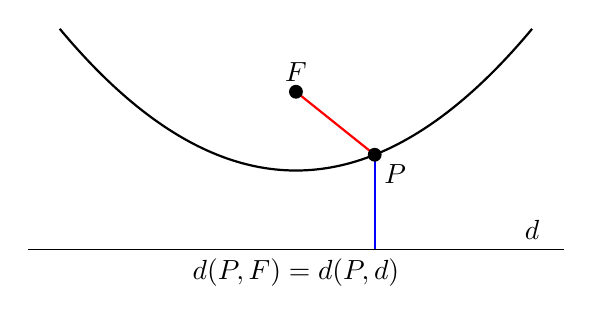
\begin{tikzpicture}[>=stealth]
    \draw[thick,domain=-3:3,samples=100] plot ({\x},{0.2*\x*\x});

    \draw (-3.4,-1)--(3.4,-1);
    \node[above] at (3,-1) {$d$};

    \draw[red, thick] (0,1)--(1,0.2);
    \draw[blue,thick] (1,0.2)--(1,-1);

    \fill (0,1)   circle (2.5pt) node[above]       {$F$};
    \fill (1,0.2) circle (2.5pt) node[below right] {$P$};

    \node[below] at (0,-1) {$d(P, F) = d(P, d)$};
  \end{tikzpicture}
  \end{center}
\end{columns}
\end{frame}

%------------------------------------------------------------------------------%
\begin{frame}{Hipérbole}
\begin{columns}
\column{0.4\textwidth}
  Uma \emph{hipérbole}

  \pause
  é o conjunto dos pontos \(P\) para os quais o módulo da
  diferença das distâncias a dois focos é constante

  \pause
  \bigskip
  Os pontos \(F_1\) e \(F_2\) são os focos
\column{0.6\textwidth}
  \begin{center}
  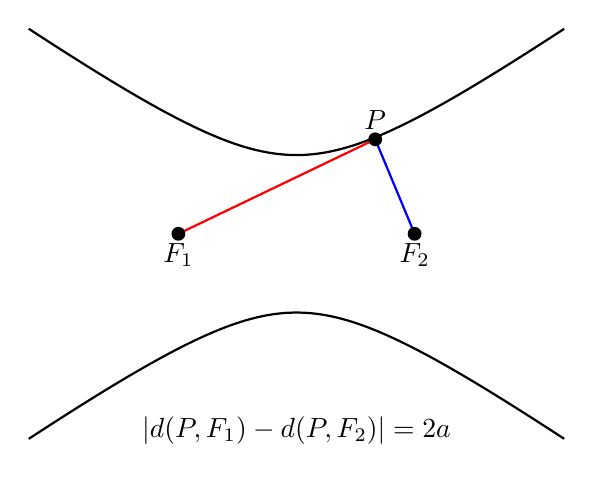
\begin{tikzpicture}[>=stealth]
    \draw[thick,domain=-3.4:3.4,samples=100] plot ({\x},{ sqrt(1+0.5*\x*\x)});
    \draw[thick,domain=-3.4:3.4,samples=100] plot ({\x},{-sqrt(1+0.5*\x*\x)});

    \draw[red, thick] (-1.5,0)--(1,1.2);
    \draw[blue,thick] ( 1.5,0)--(1,1.2);

    \fill (-1.5,0) circle (2.5pt) node[below] {$F_1$};
    \fill ( 1.5,0) circle (2.5pt) node[below] {$F_2$};
    \fill ( 1,1.2) circle (2.5pt) node[above] {$P$};

    \node at (0,-2.5) {$\left|d(P, F_1) - d(P, F_2)\right| = 2a$};
  \end{tikzpicture}
  \end{center}
\end{columns}
\end{frame}

%------------------------------------------------------------------------------%
\section{Definição Algébrica das Cônicas}

%------------------------------------------------------------------------------%
\begin{frame}{Definição Algébrica das Cônicas}
  As \emph{cônicas} são soluções de equações de segundo grau no plano

  \pause
  \[
    ax^2 + 2bxy + cy^2 + dx + ey + f = 0
  \]

  \pause
  Matricialmente
  \[
    r^tAr \;+\; B^tr \;+\; f = 0
  \]
\end{frame}

%%------------------------------------------------------------------------------%
%\section{Lista Mínima}
%
%%------------------------------------------------------------------------------%
%\begin{frame}{Lista Mínima}
%  \begin{enumerate}
%    \item
%  \end{enumerate}
%
%  \vfill
%  Atenção: A prova é baseada no livro, não nas apresentações
%\end{frame}

%------------------------------------------------------------------------------%
\end{document}
%------------------------------------------------------------------------------%
